\documentclass[11pt, oneside, fullpage, doublespace]{article}
\usepackage{geometry}                		% See geometry.pdf to learn the layout options. There are lots.
\geometry{letterpaper}                   		% ... or a4paper or a5paper or ... 
%\geometry{landscape}                		% Activate for for rotated page geometry
%\usepackage[parfill]{parskip}    		% Activate to begin paragraphs with an empty line rather than an indent
\usepackage{graphicx}				% Use pdf, png, jpg, or eps� with pdflatex; use eps in DVI mode
								% TeX will automatically convert eps --> pdf in pdflatex		
\usepackage{amssymb}

\usepackage{setspace}
\setstretch{1.5}

\title{Wireless Automobile Detection, License Plate Processing, and Data Availability Network Proposal}
\author{Kevin Emery, Santiago Gonzalez, Brandon Rodriguez, Taylor Sallee\\ \emph{Undergraduates, EECS Department, Colorado School of Mines}}
\date{March 17, 2014}




\begin{document}
\maketitle

\begin{abstract}
300 words or less. Talk about the motivation behind this project. Why it is important.
\end{abstract}

\section{Project Description}
A description

\subsection{Introduction}
Introduction. Talk about the motivation behind this project. Why it is important.

\subsection{Related Work}
\cite{stillwell2013} describes an implementation of a system to detect automobiles entering and exiting a parking lot using a magnetometer and wireless nodes based on the commercially available Arduino Fio microcontroller platform. This system uses the ubiquitous IEEE 802.15.4 communications standard to communicate automobile detection data to a central base-station based on the small, commercially available Raspberry Pi Linux computer. The project described in this proposal will augment and extend this project while collaborating closely with Stillwell, to the point of a real world deployment at the Colorado School of Mines.

\section{Proposed Work}
\subsection{Automobile Detection}
The automobile detection subsystem provides a means for detecting ingress and egress of vehicles from a parking lot. This subsystem is to be placed on the side of the road next to each parking lot entrance and exit. Automobiles will be detected using a magnetometer which perceives the induced change in the local magnetic field as the metallic structure of the vehicle passes by as described in \cite{stillwell2013}. The automobile detection subsystem will be based around the commercially available Arduino Fio 16-bit  platform which utilizes the ubiquitous Atmel ATMEGA328p microcontroller.

\begin{figure}
\begin{center}
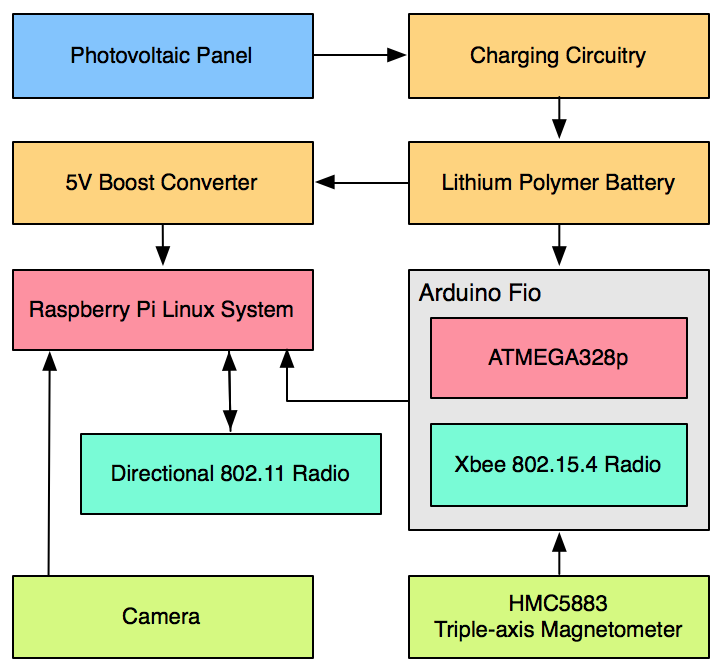
\includegraphics[width=3.5in]{autodetection}
\end{center}
\caption{Automobile Detection Subsystem Architecture}
\end{figure}

The hardware to be used for automobile detection will be contained in the same enclosure as the license plate image acquisition hardware.


The use of a magnetometer ensures that solely automobile and other large vehicles such as motorcycles are detected while pedestrians are ignored.

Work on the automobile detection subsystem will involve a variety of tests and analyses to ensure system and data integrity.


\subsection{License Plate Image Acquisition}
Kevin


\subsection{Central Basestation}
Everyone


\subsection{Server Processing}
Brandon


\subsection{Web Application}
Taylor


\subsection{Deployment}
Blah


\section{Summary}
A summary \cite{johnson2012} Talk about the motivation behind this project. Why it is important.


\begin{thebibliography}{99}
\bibitem{stillwell2013} R. Stillwell, A. Wilson ``Magnetometer Parking Sensor'' \emph{EGGN 383 Final Project, Colorado School of Mines}. December 12, 2013
\bibitem{johnson2012} X. Johnson
\end{thebibliography}





\end{document}  
